% !TEX program = xelatex

\documentclass{resume}
\usepackage{graphicx}
\usepackage{tabu}
\usepackage{multirow}
\usepackage{progressbar}
%\usepackage{zh_CN-Adobefonts_external} % Simplified Chinese Support using external fonts (./fonts/zh_CN-Adobe/)
%\usepackage{zh_CN-Adobefonts_internal} % Simplified Chinese Support using system fonts

\begin{document}
\pagenumbering{gobble} % suppress displaying page number

\Large{
  \begin{tabu}{ c l r }
   \multirow{5}{1in}{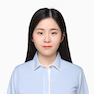
\includegraphics[width=0.88in]{resume}} & \scshape{Bao Rong} \\
    & \email{1600012979@pku.edu.cn} \\
    & \phone{(+86) 135-818-01421}\\
    \\
    \\
  \end{tabu}
}


\section{\faGraduationCap\ Education}
\datedsubsection{\textbf{Peking University (PKU)}, Beijing, China}{2016 -- Present}
\textit{Undergraduate student} in School of Electronics Engineering and Computer Science(EECS), expected June 2020


\section{\faUsers\ Research Experience}
%\datedsubsection{\textbf{e-MARS Project}}{2018 -- Present}
%\role{Supervisor: Tenjiao Wang}{}
%Brief introduction:  An Environment-Aware Market-Strategy-based System for Data Allocation and Dynamic Migration in Cloud Database
%\begin{itemize}
%  \item Participated in part of the system development work, including environmental construction and post-operational maintenance
%  \item Undertake the strategic design work in the future
%\end{itemize}

\datedsubsection{\textbf{Research in Natural Language Processing}}{Jun.2018 -- Dec.2018}
\role{Supervisor: Sujian Li}{}
Brief introduction: Chinese discourse analysis based on dependency tree
\begin{itemize}
  \item Cross-language discourse analysis based on dependency tree
  \item Using English corpus to assist Chinese discourse analysis
\end{itemize}

\datedsubsection{\textbf{Research in Data Mining}}{Jan.2019 -- Present}
\role{Supervisor: Tenjiao Wang}{}
Brief introduction: Named Entity Recognition System Based on Rule-Deep Learning Model in Medical field
\begin{itemize}
  \item Combining rule-based Named Entitiy Normalization and Deep Learning Model of Named Entity Recognition in the system
  \item Applied Named Entity Recognition System in Medical field
\end{itemize}

\datedsubsection{\textbf{Attending ICDE2019(IEEE International Conference on Data Engineering)}}{Apr.2019}
\begin{itemize}
  \item Getting the official financial grants(Chinese Student Travel Awards) to attend the conference(Top level international meeting of Databases & Data Mining) 
  \item Demonstrating the scientific research achievements and models published by our lab in the conference
\end{itemize}

% Reference Test
%\datedsubsection{\textbf{Paper Title\cite{zaharia2012resilient}}}{May. 2015}
%An xxx optimized for xxx\cite{verma2015large}
%\begin{itemize}
%  \item main contribution
%\end{itemize}

\section{\faCogs\ Internship}
\datedsubsection{\textbf{SHENZHEN CAPITAL GROUP.CO.,LTD} Beijing, China}{Dec.2018 -- Feb.2019}
Brief introduction: The intern position is investment analysts
\begin{itemize}
  \item Participating in the project due diligence and analyzing the proposed investment company
  \item Organizing relevant documents of the project and participating in the preparation of project investment documents
  \item Learning the knowledge and processes of investment projects
\end{itemize}

\section{\faHeartO\ Activities}
\datedsubsection{\textbf{Volunteer of ZhiLuYiXing letter-writing student association}}{Sept.2016-Aug.2017}
\begin{itemize}
  \item Communicate with the children from poor area, resolve their troubles and help them get in touch with better educational resources via letter-writing for a year
\end{itemize}

\section{\faInfo\ Miscellaneous}
\begin{itemize}[parsep=0.5ex]
  \item Languages: English - Fluent(TOEFL 111), Mandarin - Native speaker
  \item Programming Languages: C++、Python
\end{itemize}

%% Reference
%\newpage
%\bibliographystyle{IEEETran}
%\bibliography{mycite}
\end{document}

